\subsection{Solicitar Refacción}
En la siguiente figura \ref{fig:Diagrama de Secuencia - Solicitar Refaccion} se muestran la secuencia de las actividades que se deben de llevar a cabo para realizar la solicitud de una refacción que no se encuentre en el almacén del taller. El sistema solicita información al Mecánico (usuario) para generar una solicitud. Al ingresar datos al sistema, existe una validación de estos mismos datos, esto lleva al sistema a tomar dos caminos: 
\begin{itemize}
	\item \textbf{Información válida:} Los datos ingresados por el usuario son válidos, el formato y los campos han sido llenados correctamente de acuerdo a los datos que el sistema solicite.  
	\item \textbf{Información no válida:} Los datos ingresados por el usuario no son válidos, los campos o el formato no son correctos y el sistema muestra un mensaje de error.
\end{itemize} 
\begin{figure}[!h]
	\centering
	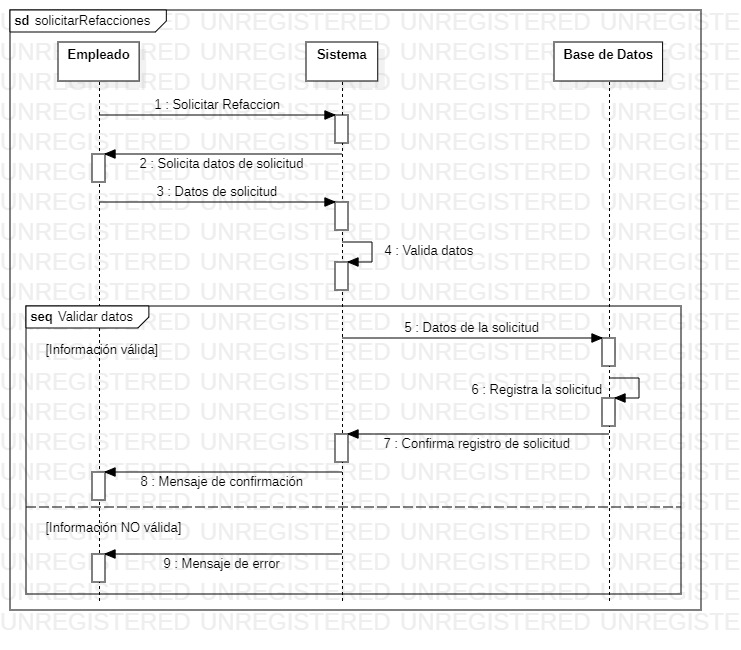
\includegraphics[width=0.9\textwidth]{./diseno/vprocesos/imagenes/solicitarRefacciones}
	\caption{Diagrama de Secuencia - Solicitar Refacción}
	\label{fig:Diagrama de Secuencia - Solicitar Refaccion}
\end{figure}
\clearpage